\section {Evaluation}
\label{sec:results}

We evaluated the effectiveness of our method on supporting juxtaposed visual comparisons by comparing it against existing methods across different visualization types.
Considering that oftentimes there are multiple tasks involved in juxtaposed visual comparisons, we evaluated our method from two different perspectives, i.e., examining how well it can support people  (1) to \emph{observe the changes} for juxtaposed categorical visualizations (i.e., identifying delta), and (2) to \emph{visually distinguish different classes} in each individual visualization in the pair (i.e., identifying the number of classes being compared), which is considered fundamental to juxtaposed comparison~\cite{Gleicher18}.
Besides, we also examined whether the effect of our method would be consistent across different visualization types by applying it to two charts: bar charts and scatterplots, which are typical and widely-used examples of statistical graphics.

To achieve these evaluation goals, we conducted three online controlled experiments through Amazon Mechanical Turk (AMT) involving 30 participants for one bar chart task (replicating Ondov et al.'s~\cite{Ondov19} study) and 160 participants for two scatterplot tasks respectively, and in each we compared \emph{$C^3$-palette} with existing benchmark methods.

%In each experiment we evaluated one visualization type using the tasks listed below:
%\begin{enumerate}
%%\vspace{-3mm}
%\item [(i)] Experiment 1: Bar chart experiment:
%    \begin{itemize}
%         \item \emph{Finding max delta task}. To evaluate how well our method can support people in \emph{observing the largest change} for juxtaposed categorical bar charts;
%    \end{itemize}
%%\vspace{-3mm}
%\item [(ii)] Scatterplot experiment:
%    \begin{itemize}
%         \item \emph{Spotting the difference task}. To evaluate how well our method can support people in \emph{observing changes} for juxtaposed categorical scatterplots;
%         \item \emph{Counting class number task}. To evaluate whether our method can support the \emph{visual separability} in each individual scatterplot, which is considered fundamental to juxtaposed comparison.
%    \end{itemize}
%\end{enumerate}
%we use synthetic data for the first three studies while use real world data for the case study.

\vspace{.3em}
\noindent{\textbf{Colorization Methods (Conditions).}} In each of our experiments, we compared six different colorization methods, specifically including four benchmark methods (\emph{Random Assignment}, \emph{Optimized Assignment}~\cite{Wang2018}, \emph{Alpha Blending} and \emph{Palettailor}~\cite{Lu21}) that colorize based on one of the two input datasets, and our approach (\emph{$C^3$-palette Assignment}, \emph{$C^3$-palette Generation}) that colorize based on both input datasets. The first three methods are based on Tableau 20~\cite{tableau}, which is a designer-crafted palette containing colors with a large range of brightness and saturation, and the other three methods are generating and assigning colors to classes automatically. These methods are ordered by the level of optimization applied.
\begin{enumerate}
     \item \emph{Random Assignment:} This is the common default result in data visualization by randomly selecting and assigning colors from a given palette to one of the two datasets.
     \item \emph{Optimized Assignment:} Using the optimal discrimination assignment approach~\cite{Wang2018} to mimic the best discriminable result from user manual selection with a proper palette. This is achieved by selecting and assigning colors from the given palette to one of the two datasets. Since the original method was designed for scatterplots,  we extend it for bar charts by treating each bar as a point in scatterplots as Lu et al.~\cite{Lu21}.
        % applied to the bar chart in~\cite{Wang2018} . We applied their method in our experiment by extending the approach, i.e., treating each bar as a point and then computing the bar chart as a scatterplot.
     \item \emph{Alpha Blending:} This is the straightforward way to highlight classes: setting the unchanged classes to be semi-transparent (i.e., $alpha=0.5$) while keeping the changed classes to be opaque. We choose the $0.5$ threshold through empirical tests to balance between saliency and discriminability among classes. We applied this method to \emph{Optimized Assignment} result to improve the discriminability of different classes.  %\mf{Question: can we use "empirical tests" to justify the choice of 0.5 here?}
     \item \emph{Palettailor:} Since this is the state-of-the-art palette generation method for single view colorization, we used \emph{Palettailor}~\cite{Lu21} to generate and assign colors based on one of the two datasets with the default settings.
     \item \emph{$C^3$-palette Assignment:} Selecting and assigning colors from the Tableau-20 palette based on \emph{both} datasets as input, using the color assignment optimization solution (Eq.~\ref{eq:cosaliency}) proposed in this paper. This condition aims to reflect the effectiveness of our assignment approach given a palette input with relatively diverse options, such as Tableau-20.
     \item \emph{$C^3$-palette Generation:} Generating colors using the color generation method (Eq.~\ref{eq:energyfunc}) with the default settings ($\omega_0=1.0$, $\omega_1=1.0$, $\omega_2=1.0$ and $\kappa=0$). This condition aims to reflect the effectiveness of the fully automated option of our method.
\end{enumerate}
%\emph{Change magnitude}: While the colorization method is the primary independent variable to be investigated, we are also interested in how the effect of different methods would vary based on the level of change between the two scatterplots. Thus we first define two types of changes that a class would have across multiple scatterplots: \emph{point number} and \emph{point position}. Then for each change type, we define three levels of change magnitude calculated using Eq.~\ref{eq:cm}: \emph{small}, \emph{medium}, and \emph{large}. (See the next paragraph for the detailed calculation.)


\subsection{Experiment 1: Bar Chart Experiment}
\label{subsec:barchartExp}
We evaluated the effectiveness of our method on supporting juxtaposed visual comparisons using bar charts by following Ondov et al.'s~\cite{Ondov19} comparison evaluation, in which the participants performed the \emph{max delta task}. The \emph{max delta task} can reflect how well our method can support people to \emph{observe the changes} for juxtaposed comparisons. We did not evaluate the other perspective: discriminating classes in individual charts, because the task is considered trivial in the context of bar chart, and so that it could lead to ceiling effect.

For the \emph{max delta task}, we hypothesized that our method would generally be more effective than the benchmark methods on the task performance, and specifically we had the following hypotheses:
\begin{itemize}[noitemsep]
\setlength{\itemsep}{5pt}
    \item[\textbf{H1.}] Our palette generation method (\emph{$C^3$-palette Generation}) outperforms the benchmark conditions (\emph{Random Assignment}, \emph{Optimized Assignment}, \emph{Alpha Blending} and \emph{Palettailor}) on the task performance.
    \item [\textbf{H2.}] Our color assignment method (\emph{$C^3$-palette Assignment}) using a color palette with a large range of brightness and saturation (\emph{Tableau-20}) outperforms the benchmark conditions (\emph{Random Assignment}, \emph{Optimized Assignment}, \emph{Alpha Blending} and \emph{Palettailor}) on the task performance.
\end{itemize}

\noindent{\textbf{Task \& Measures. }
Following the methodology by Ondov et al.~\cite{Ondov19}, we asked the participants perform the \emph{max delta task}
%, or finding the maximum delta task
. Specifically, the participants were asked to find the bar that had the largest difference in the two bar charts.
%The titer value which is used to control the largest difference between the two bar charts, is recorded to measure the precision degree for people to make judgments about adjacent bar charts. Larger titer value indicates an easier trial. In addition to titer value (ranging from 0 to 1), we also record the answer, where a correct response recorded as 1 and wrong is 0.
For each trial, we measured the \emph{titer value} (ranging from 0 to 1) and \emph{error} (using 0 and 1) to evaluate the performance of different conditions.
% and the time taken to complete it \lk{the time is not recorded since each trial is displayed in 1.5s and the time to complete it might be meaningless}.

\noindent{\textbf{Dataset generation. }}
All the stimulus datasets used in this experiment were generated by the titer staircase method~\cite{Ondov19} in real time, where each bar chart in the pair consisted of 7 data points (bars), and each pair of bar charts were generated differently depending on participant performance in the previous trial. This was done in order to minimize the learning effect. Specifically, we used \emph{titer value}~\cite{Ondov19}, the largest difference between the two bar charts, to quantify and control the difficulty of a trial. A larger titer value indicates an easier trial. For each condition method, the first trial contains the bar chart pair with a titer of $0.5$. An erroneous response made the titer of the next trial increase by $0.3$ (easier) while a correct answer led to a decrease by $0.1$ (harder). We set $0.75$ as the maximum titer value to prevent participants from going through too many easy trials.

%\noindent{\textbf{Sample palettes for the conditions. }}
%We generated the sample palettes for each of the six conditions using their respective methods. For more details about this process please see the supplementary materials. Here we note a few special points. First, for the \emph{Optimized Assignment} condition, in the original paper~\cite{Wang2018} the method was not applied to a bar chart. We applied their method in our experiment by extending the approach, i.e., treating each bar as a point and then computing the bar chart as a scatterplot. Second, we ran the six methods in real-time and generated bar charts dynamically following Ondov et al.~\cite{Ondov19}, instead of pre-computing all the palettes.

\noindent{\textbf{Procedure. }}
Prior to the main task, each participant viewed the instructions and went through four training trials. The first training trial does not have a time limit and the participant has to answer correctly in order to pass, while the other three trials are identical to the real test (having a time limit of 1.5 seconds for impression) with the largest titer value ($0.75$), i.e., easiest trials. Then each participant had $120$ trials in the main study, i.e., twenty trials for each condition methods. The order of the conditions was randomized. All the bar charts are generated dynamically and the method conditions are run in real-time.

\vspace{.3em}
\noindent{\textbf{Participants.}}
We recruited 32 participants through the Amazon Mechanical Turk, and each participant went through all the six condition methods with random order.
According to the completion time in the pilot study, we paid each participant \$$1.5$ for the task based on the US minimum hourly wage.
No participant claimed color vision deficiency on their informed consent.


\noindent{\textbf{Analysis. }}
We ran an accuracy-based outlier exclusion to filter participants whose overall proportion of correct trials was lower than two standard deviations from the mean of that from the other participants. This procedure resulted in 2 participants being excluded from the analysis. Following Ondov et al.~\cite{Ondov19}, we performed within-subjects comparisons of the means of the \emph{titer values} of the final 5 trials per condition. Aside from this primary indicator of the task performance, we also compared the \emph{error} measure in a similar manner as a secondary indicator. Specifically, for each measure, we calculated the 95\% confidence intervals using the bootstrap method. In addition, we used the more conservative, non-parametric Wilcoxon signed-rank test without normality assumption to compare different condition groups.

\begin{figure*}[!tb]
\centering
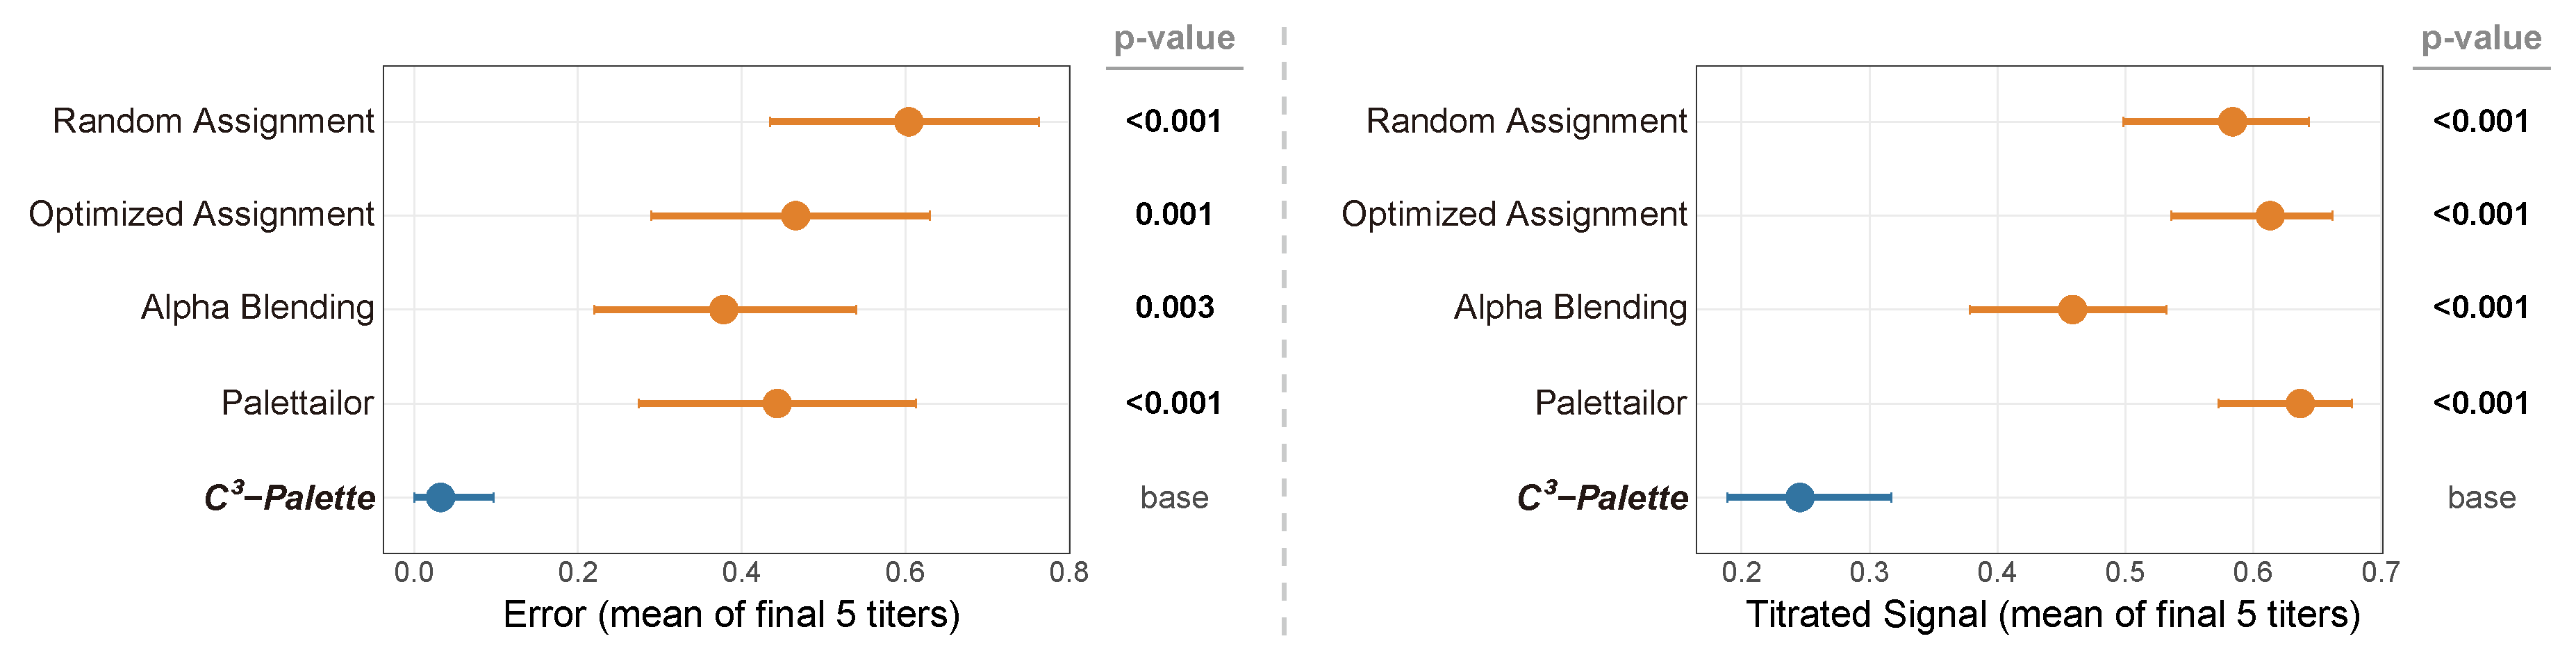
\includegraphics[width=1\linewidth]{figures/maxdelta-results.pdf}
\caption{Confidence intervals and p-values from the Mann-Whitney test for the \emph{max delta task} of the bar chart experiment. Error bars represent $95\%$ confidence intervals. Each p-value shows the statistical test result of one base with the other conditions. Smaller value means a better performance.}
\vspace*{-3mm}
\label{fig:barResults}
\end{figure*}
\noindent{\textbf{Results. }}
As shown in Fig.~\ref{fig:barResults}, the condition method \emph{$C^3$-palette Generation} led to a significantly better task performance (indicated by lower \emph{Titrated Signal} and \emph{Error}) compared to the benchmark conditions ($p<0.001$). (\textbf{H1} confirmed)
Similarly, the condition method \emph{$C^3$-palette Assignment} also led to a significantly better task performance (indicated by lower \emph{Titrated Signal}) compared to the benchmark conditions: \emph{Random Assignment} ($p<0.001$), \emph{Optimized Assignment} ($p<0.001$), \emph{Alpha Blending} ($p=0.005$), \emph{Palettailor} ($p<0.001$). (\textbf{H2} confirmed) Please see the supplementary materials for the detailed statistics.




\subsection{Experiment 2: Scatterplot Experiment}
\label{subsec:scatterplotExp}
In addition to bar charts, we also evaluated our approach in a more complex visualization scenario -- scatterplots, where different visual tasks are involved that need to be supported.
Specifically, we evaluated whether our method can support people to \emph{observe the changes} for juxtaposed categorical scatterplots, as well as to \emph{visually distinguish different classes} in each individual scatterplot.
Therefore we adopted two tasks from literature: the \emph{identifying delta task}~\cite{Fukuba2009} and \emph{counting class task}~\cite{Lu21} to reflect the performance of the two perspectives.
In addition, in this experiment we also examined whether the effect of our method would vary based on \emph{change magnitude}, the magnitude of the change between two scatterplots.

For the two tasks, we applied the similar experiment design and used the same set of pre-defined datasets, while recruited different groups of participants. Thus we describe the dataset generation and experiment organization altogether and report the results separately.


\vspace{.3em}
\noindent{\textbf{Dataset Generation.}}
The paired scatterplot datasets used in our studies were generated as follows.
First, we generated a set of multi-class scatterplots, each containing $8$ classes. Each class was generated using Gaussian random sampling and placed randomly in a $600 \times 600$ area.
Similar to~\cite{Lu21}, these classes belong to one of the four settings of varying size and density: small \& dense ($n=50, \sigma=20$), small \& sparse ($n=20, \sigma=50$),  large \& dense ($n=100, \sigma=50$), and large \& sparse ($n=50, \sigma=100$).

For each scatterplot generated above, we produced its paired scatterplot by randomly changing one or more of its classes.
To systematically changing the classes, we defined \emph{change magnitude} which quantifies the magnitude of change between two scatterplots using Eq.~\ref{eq:cm}. We generated scatterplot pairs with three levels of change magnitude: small, medium and large, by varying three underlying factors: \emph{change type}, \emph{change ratio} and \emph{number of changed classes}.
\emph{Change type} defines \emph{how} the points in a class change. There are two types of changes: \emph{point number change}, where the number of points in a class changes, and \emph{point position change}, where the positions of the points in a class change.
\emph{Change ratio} defines \emph{how large} the change of a type is, ranging from 0 to 1. {Number of changed classes} defines \emph{how many} classes are changed, ranging from 1 to 3.

For each change type, we report the process in which the changes were generated.
First, for the \emph{point number} change type, we calculated the new point number by adding or subtracting points from the original class by ($1 \pm$ \emph{change ratio}), where the additional points were generated with the same distribution as that for the original class, and the subtraction of points was achieved by randomly deleting data points from the original class.
Second, for the \emph{point position} change type, we randomly chose from two kinds of positional changes: moving the \emph{center} of the entire class, and moving the individual point positions, which results in the change of the \emph{shape} of the class. For the \emph{center} change, we moved the center towards a random direction by a distance, which equals to a maximal distance ($400$ by default) weighted by \emph{change ratio}. For the \emph{shape} change, we moved the density parameter of its Gaussian distribution into the opposite direction of the given value. For example, a small \& dense class ($n=50, \sigma=20$) would be changed into a small \& sparse ($n=50, \sigma=50$) class. After calculating the one-to-one mapping between the new and original class using ~\cite{kuhn1955hungarian}, we linearly interpolated the position for each point weighted by \emph{change ratio}.

From the above process, we produced 300 candidate scatterplot pairs for each change type, and then calculated the \emph{change magnitude} for each pair using Eq.~\ref{eq:cm}, and split all  pairs into three levels: \emph{small}, \emph{medium}, and \emph{large}.
Finally, without loss of fairness, we randomly selected $2$ pairs from each change magnitude level for each change type and each number of changed classes. Thus in total we had $36$ scatterplot pairs. The detailed dataset is showed in Fig.~\ref{fig:experimentOrgan} (a).%Table.~\ref{tab:latinsquare}.
%
%\begin{table}[ht]
%     \renewcommand\arraystretch{1}
%     \centering
%     \caption{Grouping of Datasets: $36$ datasets $\times$ $6$ conditions. C: condition; G: participant group; Position Small 1: point position change with small change magnitude for 1 changed class.}
%     \label{tab:latinsquare}
%     \begin{tabular}{lcccccccc}
%     \hline
%      & C1 & C2 & C3  & C4 & C5 & C6 \\
%
%     \hline
%     Dataset 1: Position Small 1 & \textbf{G1} & G2 & G3  & G4 & G5 & G6 \\
%     Dataset 2: Position Small 1 & G6 & \textbf{G1} & G2 & G3  & G4 & G5 \\
%     Dataset 3: Position Small 2 & G5  & G6 & \textbf{G1} & G2 & G3 & G4 \\
%     Dataset 4: Position Small 2 & G4 & G5  & G6 & \textbf{G1} & G2 & G3 \\
%     Dataset 5: Position Small 3 & G3 & G4 & G5  & G6 & \textbf{G1} & G2 \\
%     Dataset 6: Position Small 3 & G2 & G3 & G4  & G5 & G6 & \textbf{G1} \\
%     Dataset 7: Position Medium 1 & \textbf{G1} & G2 & G3  & G4 & G5 & G6 \\
%     Dataset 8: Position Medium 1 & G6 & \textbf{G1} & G2 & G3  & G4 & G5 \\
%     ... & & & & & & &\\
%     Dataset 35: Number Large 3 & G3 & G4 & G5  & G6 & \textbf{G1} & G2 \\
%     Dataset 36: Number Large 3 & G2 & G3  & G4 & G5 & G6 & \textbf{G1}  \\
%
%     \hline
%     \end{tabular}
%\end{table}

\vspace{.3em}
\noindent{\textbf{Experiment Organization.}}
We did not follow the \emph{within-subject}  experiment design as the above experiment, since it will inevitably introduce the learning effect with 216 trials (6 conditions and 36 datasets) for each participant.
Instead, we adopted  a \emph{between-subject} experiment design to test the effects on scatterplots.
To avoid ordering effects, where the participant would get familiar with a dataset after seeing it several times (six times in our case), each participant was assigned to a group and saw a specific subset of datasets under different conditions. We used a Latin Square grouping (see Fig.~\ref{fig:experimentOrgan} (a)) to organize the trials for each participant. %$Thus, there were $6$ participant groups and each of them had $40$ trials in total. See the supplementary material for more details.

For attention check, we added four additional validation stimuli for both tasks. Each stimulus has a pair of scatterplots with 6 well-separated classes, including only one changed class with a large change magnitude, and we assigned a de-saturated color to the changed class that made it less salient. Accordingly, there are $36+4 = 40$ trials in total for each participant group. To alleviate learning effects, we randomly shuffled the display orders of all scatterplot pairs, and randomly placed the two scatterplots in each pair on the left or right side.

 %We add these 4 distractor trials to each group to identify whether the participant is doing the task seriously and reject the results with more than two wrong trials.

%during some participants might apply a ``shortcut'' strategy when seeing a class that is obviously more salient than the others, especially under the \emph{$C^3$-palette} condition.
%And for \emph{counting class task}, some participants might simply select 8 for all trials since they find many simple trials are 8 classes.
%Thus, for quality control, we added $4$ sentinels which were very simple trials with 6 classes, including only one changed class with a large change magnitude, and we assigned a de-saturated color to the changed class that made it less salient. All the classes are well separated. We add these 4 distractor trials to each group to identify whether the participant is doing the task seriously and reject the results with more than two wrong trials.


\begin{figure*}[h]
\centering
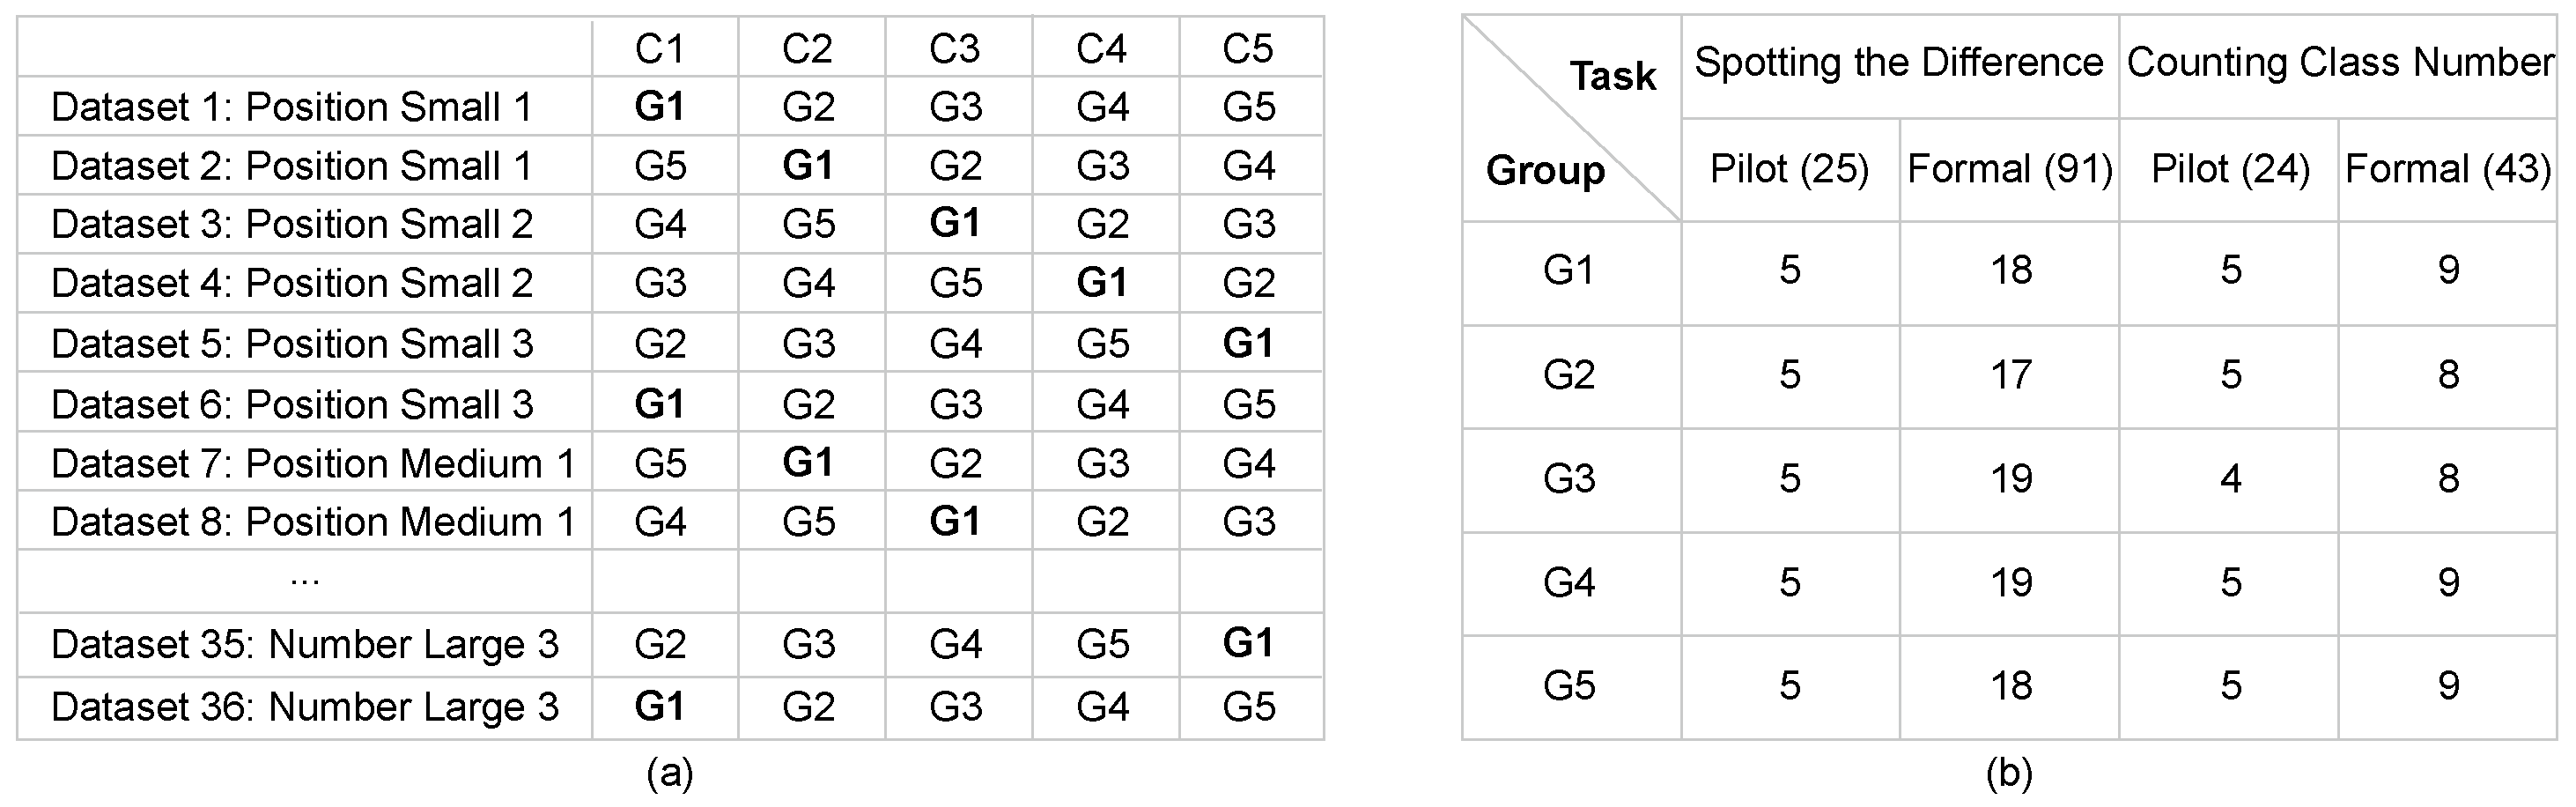
\includegraphics[width=1\linewidth]{figures/experiment-organization.pdf}
\caption{Experiment organization for the scatterplot experiment. (a) Grouping of Datasets: $36$ datasets $\times$ $6$ conditions. C: condition; G: participant group; Small (Position, 1): point position change with small change magnitude for 1 changed class; (b) Participants details for each task of the scatterplot experiment.}
\vspace*{-3mm}
\label{fig:experimentOrgan}
\end{figure*}

\subsubsection{Identifying delta task}
\
\newline
To evaluate how well our approach enables viewers observing changes between juxtaposed categorical scatterplots, we conduct an online \emph{identifying delta} experiment through Amazon Mechanical Turk (AMT) with 108 participants.
%We show participants a set of paired multi-class scatterplots, and ask them to find a known number of classes that have been changed within $60$ seconds.  Error rate and consuming time are recorded for analysis.
%This task is inspired by the ``Spot the Difference'' game where one needs to compare a pair of similar pictures to detect their differences~\cite{Fukuba2009},
In this task, we asked participants to identify all the classes that have been changed between two scatterplots.

\vspace{.3em}
\noindent{\textbf{Hypotheses.}} We hypothesized that our approach would generally be more effective than the benchmark methods on the juxtaposed comparison tasks, and that this effect would vary based on \emph{change magnitude}.
%In this experiment, our major goal is to investigate if our co-saliency based color design formulation would affect the performance of observing changes between multiple datasets.
\begin{itemize}[noitemsep]
\setlength{\itemsep}{5pt}
    \item[\textbf{H1.}] Our palette generation method (\emph{$C^3$-palette Generation}) outperforms the benchmark conditions (\emph{Random Assignment}, \emph{Optimized Assignment}, \emph{Alpha Blending} and \emph{Palettailor}) on the task performance.

    \item [\textbf{H2.}] Our color assignment method (\emph{$C^3$-palette Assignment}) using a color palette with a large range of brightness and saturation (\emph{Tableau-20}) outperforms the benchmark conditions (\emph{Random Assignment}, \emph{Optimized Assignment}, \emph{Alpha Blending} and \emph{Palettailor}) on the task performance.

    \item [\textbf{H3.}] There is a significant interaction effect between colorization methods and \emph{change magnitude}, resulting that the performance of our methods (\emph{$C^3$-palette Generation} and \emph{$C^3$-palette Assignment}) and that of the benchmark methods (\emph{Random Assignment}, \emph{Optimized Assignment}, \emph{Alpha Blending} and \emph{Palettailor}) vary based on \emph{change magnitude}.
\end{itemize}

\vspace{.3em}
\noindent{\textbf{Measures.}}
For each participant, we measured the \emph{time} taken for each trial, and counted the errors ($0/1$) indicating whether the actual changed classes are aligned with the participant's response. Note that if any of the changed classes was mistakenly identified, the trial would be considered as ``wrong'' (1).



%\begin{table}[ht]
%\renewcommand\arraystretch{1}
%\centering
%\caption{Participants details for each task of the scatterplot experiment.}
%\label{tab:participantDetail}
%\begin{tabular}{|c|c|c|c|c|}
%\hline
%\multirow{2}{*}{\textbf{Task \& Group}} & \multicolumn{2}{c|}{Spotting the Difference} & \multicolumn{2}{c|}{Counting class number} \\
%\cline{2-5}
%& Pilot(28) & Formal(108) & Pilot(29) & formal(52) \\
%\hline
%Group 1 & 5 & 18 & 5  & 9 \\
%\hline
%Group 2 & 5 & 17 & 5  & 8 \\
%\hline
%Group 3 & 5 & 19 & 4  & 8 \\
%\hline
%Group 4 & 3 & 17 & 5  & 9 \\
%\hline
%Group 5 & 5 & 19 & 5  & 9 \\
%\hline
%Group 6 & 5 & 18 & 5  & 9 \\
%\hline
%\end{tabular}
%\end{table}


\vspace{.3em}
\noindent{\textbf{Pilot Study.}} %\& Power Analysis.}}
We conducted a pilot study involving 28 participants to check the experimental setup and determine the parameters, such as the time limit for a trial.
Harnessing by the pilot study, we also obtained our expected effect sizes, which were in further fed into a power analysis. With an effect size Cohen's $d$ of $0.4$, alpha level of $0.05$ and beta level of $0.8$, the power analysis suggested a minimum number of $100$ participants for the spot-the-difference task. See the supplementary material for more details.


\vspace{.3em}
\noindent{\textbf{Participants.}}
We recruited $108$ participants (see Fig.~\ref{fig:experimentOrgan} (b)) for the experiment on Amazon Mechanical Turk.
According to the completion time in the pilot study, we paid each participant \$$1.5$ for the task based on the US minimum hourly wage.
No participant claimed color vision deficiency on their informed consent.

\vspace{.3em}
\noindent{\textbf{Procedure.}}
Each participant went through the following steps in our experiment: (i) viewing a user guide of the task and completing three training trials; (ii) completing each trial as accurately as possible; (iii) providing demographic information. At the beginning of each trial, the number of changed classes was provided. Each participant was asked to select all the changed classes by clicking one of the points belonging to these classes in either of the scatterplots. While the participant was instructed to do the task ``\emph{as accurately as possible}'', we set a $60$-second time limit for each trial for fear that user might spend too much time on the trial. If the participant could not find all the changed classes during the time limit, they were directed to the next trial. %There also will appear a ``\emph{Can't Find it}'' button after $30$ seconds.
This was done since we observed from the pilot study that when participants spent too much time on a single trial, they may decide to quit by selecting a class randomly (which would lead to an incorrect answer) or to spend more time till they get the correct answer
%or the time limit would kick in
(which would lead to an increasing time spent on the trials). Such subject decisions would add noise to our measurements. Thus we added a $60$-second time limit, which was indicated by our pilot study: over $92\%$ of the trials were completed within that time.

%\subsubsection{Results}
%\
%\newline
\noindent{\textbf{Analysis. }}
Following previous studies, we analyzed the results using 95\% confidence intervals, and also conducted Mann-Whitney tests to compare the differences between conditions. The non-parametric test was used due to observations of non-normally distributed data from our pilot study. In addition, we computed the effect size using \emph{Cohen's d}, i.e., the difference in means of the conditions divided by the pooled standard deviation. We calculated ANOVA-type statistic (ATS) without normality assumption (using R Package GFD~\cite{gfd2017} to examine the interaction effect between variables.


\noindent{\textbf{Results. }}
Fig.\ref{fig:difference-results} shows the results of the online experiment.
First, we found that our approach \emph{$C^3$-palette Assignment} leads to a significantly lower error rate than all benchmark conditions: \emph{Random Assignment} ($p<0.001$), \emph{Optimized Assignment} ($p<0.001$), \emph{Alpha Blending} ($p=0.005$), \emph{Palettailor} ($p=0.002$). \emph{$C^3$-palette Generation} also has a significantly lower error rate than all benchmark conditions: \emph{Random Assignment} ($p<0.001$), \emph{Optimized Assignment} ($p<0.001$), \emph{Alpha Blending} ($p=0.007$), \emph{Palettailor} ($p=0.003$).
The results for the completion time also shows a similar trend of our methods taking significantly less time than the benchmarks, with an exception that \emph{$C^3$-palette Assignment} has no significant difference to \emph{Alpha Blending} condition.
The result indicates that our palette generation method (\emph{$C^3$-palette Generation}) has a better performance than benchmark conditions in the \emph{identifying delta task} (\textbf{H1} confirmed). As for color palettes with a larger range of brightness and saturation, our approach (\emph{$C^3$-palette Assignment}) is better than the benchmark conditions in terms of error rate and is better than most benchmark conditions on completion time (\textbf{H2} partially confirmed).

\begin{figure*}[!tb]
\centering
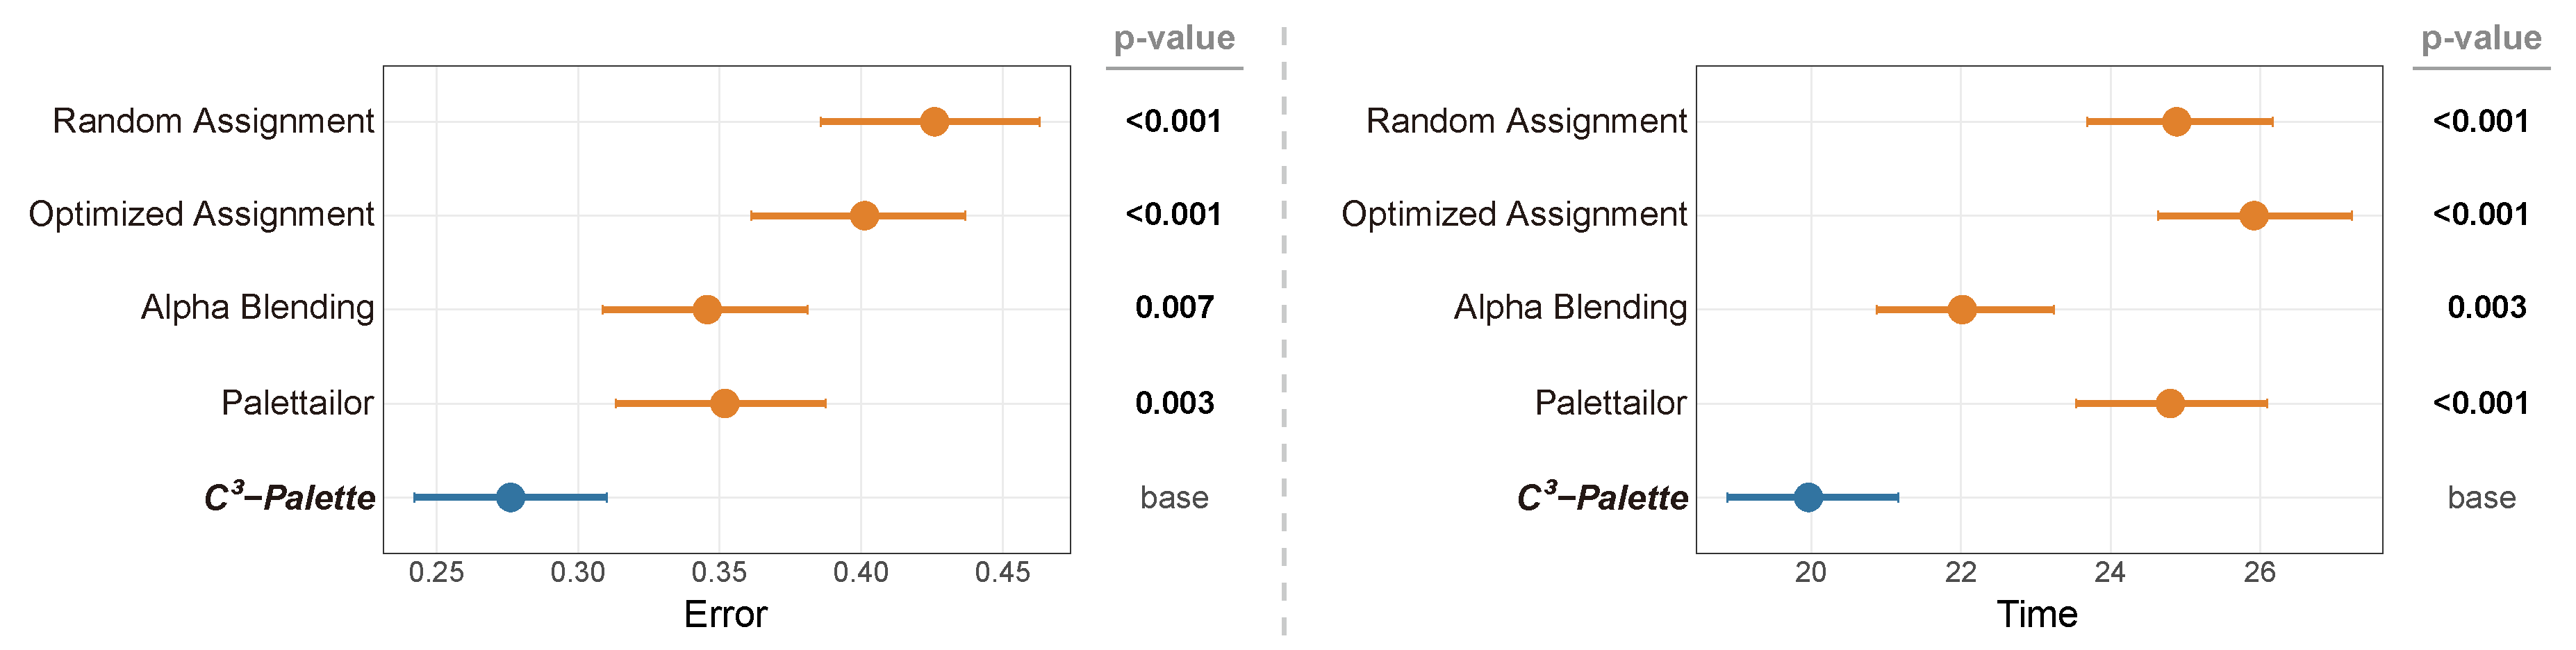
\includegraphics[width=1\linewidth]{figures/difference-results.pdf}
\caption{Confidence intervals and p-values from the Mann-Whitney test for the \emph{identifying delta task} of the scatterplot experiment. Error bars represent $95\%$ confidence intervals. Each p-value shows the statistical test result of one base with the other conditions. Smaller value means a better performance.}
\vspace*{-3mm}
\label{fig:difference-results}
\end{figure*}


%Second, we compared our approach to other conditions based on two different change types(\emph{Point Number Change} and \emph{Point Position Change}).
%For \emph{Point Number Change}, as shown in the top row of  Fig.\ref{fig:userResults} (c), our approach(\emph{C3-Palette Assignment} and \emph{C3-Palette Generation}) leads to a significantly lower error rate than all benchmark conditions, including \emph{Random Assignment} and \emph{Optimized Assignment}(\emph{$p < 0.001$}), \emph{Alpha Blending} and \emph{Palettailor}(\emph{$p < 0.05$}). \emph{C3-Palette Generation} condition has a better performance on consuming time than all other benchmark conditions, while \emph{C3-Palette Assignment} is just comparable to \emph{Alpha Blending} condition.
%For \emph{Point Position Change}, we observed that our approach has significant lower error rate than \emph{Random Assignment} and \emph{Optimized Assignment}(\emph{$p < 0.01$}), while there's no significant difference with \emph{Alpha Blending} and \emph{Palettailor}. \emph{C3-Palette Generation}) leads to a significantly lower consuming time than all benchmark conditions(\emph{$p < 0.001$}) except \emph{Alpha Blending}(\emph{$p = 0.044$})(\textbf{H3} confirmed).

%Second, we compared error and time with regard to different change magnitudes, and found that smaller magnitude leads to larger error rate and consuming time (as shown in Fig.\ref{fig:userResultsVar} (a) left). This indicates that there exists an significant interaction effect between \emph{change magnitude} and performance, i.e., \emph{change magnitude} would affect user performance. We did the same test to \emph{change type}, the results show that \emph{point number change} is much more difficult than \emph{point position change}(\textbf{H3} confirmed).

However, we did not find significant interaction effect between \emph{colorization methods} and \emph{change magnitude} ($F(5, 3876) = 1.036; p>0.05$), meaning that the effect of our method is not necessarily influenced by the magnitude of change between the two scatterplots (\textbf{H3} not confirmed).

%\begin{figure*}[h]
%\centering
%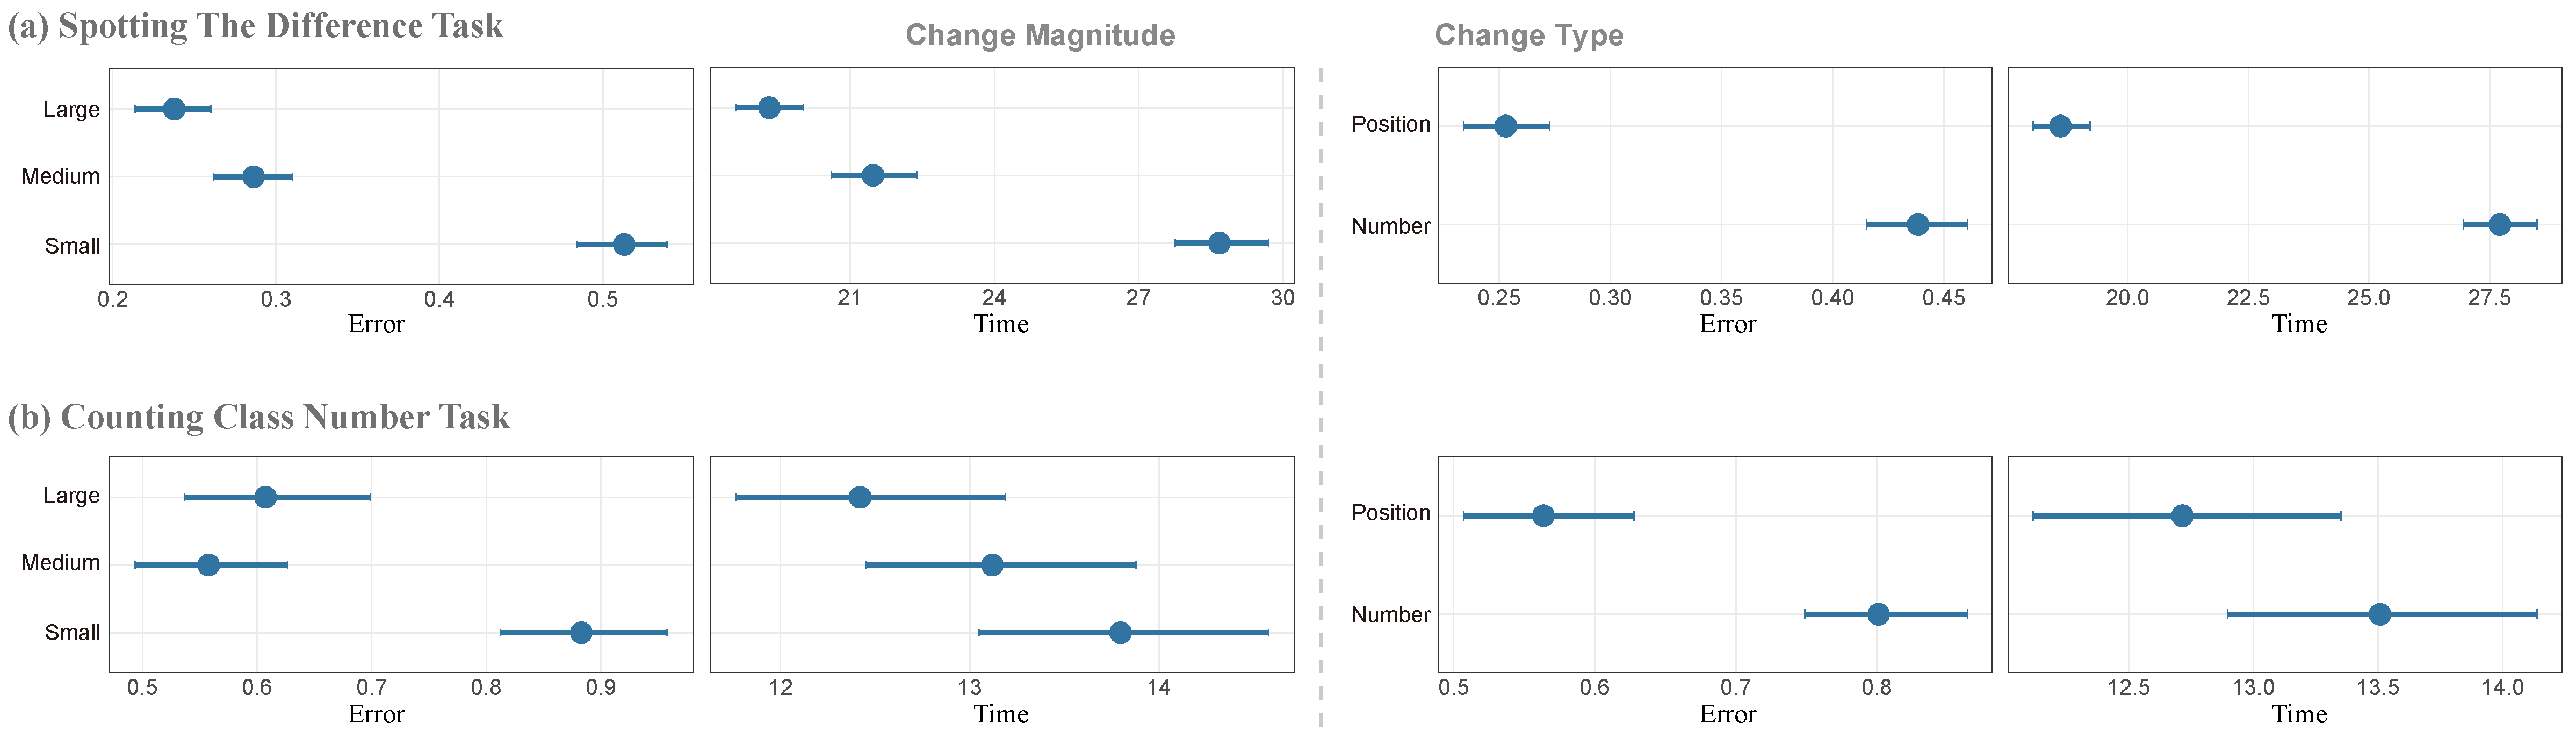
\includegraphics[width=1\linewidth]{figures/user-result-formal-variables.pdf}
%\caption{Confidence interval plots for the two online controlled experiments. (left) Plots for \emph{change magnitude} based on error and time; (right) plots for \emph{change type} based on error and time.\lk{This might be moved to supplemental material.}}
%\vspace*{-3mm}
%\label{fig:userResultsVar}
%\end{figure*}

\subsubsection{Counting class task}
\
\newline
To evaluate whether our approach can fundamentally support the visual separability of the classes in each scatterplot, we conducted an online \emph{counting class} experiment through AMT with 52 participants. Following previous methodologies~\cite{Wang2018, Lu21}, we asked participants to identify how many classes (colors) are there in the given two scatterplots and then choose an answer among several options below the two scatterplots. The experimental design was similar to the first study.
We expected to see different patterns of the discriminability across different conditions. Specifically, our methods would lead to a shorter error and time than \emph{Random Assignment} and \emph{Alpha Blending} conditions.

\vspace{.3em}
\noindent{\textbf{Hypotheses.}} We hypothesized that our approach would generally be more effective than the benchmark methods on the discrimination tasks, and that this effect would vary based on \emph{change magnitude}. %Since this task need participant count the class number in each scatterplot and two of the benchmark methods are designed for discriminable colorization,
We proposed different hypotheses with the previous task.
\begin{itemize}[noitemsep]
\setlength{\itemsep}{5pt}
    \item[\textbf{H1.}] Our palette generation method (\emph{$C^3$-palette Generation}) outperforms the benchmark conditions (\emph{Random Assignment}, \emph{Optimized Assignment}, \emph{Alpha Blending}) and our assignment method (\emph{$C^3$-palette Assignment}), while is not worse than the state-of-the-art single view discriminable colorization method (\emph{Palettailor}) on the task performance.

    \item [\textbf{H2.}] Our color assignment method (\emph{$C^3$-palette Assignment}) based on \emph{Tableau-20} outperforms the conditions (\emph{Random Assignment}, \emph{Alpha Blending}), and is not worse than the state-of-the-art single view discriminable assignment method (\emph{Optimized Assignment}) on the task performance, since all of these methods take into account the class separability.

    %    . \mf{Need to explain why the hypothesis is different from that for the first task}.

    \item [\textbf{H3.}] There is a significant interaction effect between colorization methods and \emph{change magnitude}, resulting that the performance of our methods (\emph{$C^3$-palette Generation} and \emph{$C^3$-palette Assignment}) and that of the benchmark methods (\emph{Random Assignment}, \emph{Optimized Assignment}, \emph{Alpha Blending} and \emph{Palettailor}) vary based on \emph{change magnitude}.
\end{itemize}

\vspace{.3em}
\noindent{\textbf{Measures. }}
We recorded the participant's answer and response time for each trial, and counted the \emph{error}  by calculating the differences between the participant's answer and the actual number of classes.


\vspace{.3em}
\noindent{\textbf{Pilot Study.}} %\& Power Analysis.}}
This setting is similar to the previous task. We invited $29$ participants to do the pilot study and the results were in further fed into a power analysis. With an effect size Cohen's $d$ of $0.6$, the power analysis suggested a minimum number of $50$ participants for the discriminability task.  See the supplementary material for more details.

\vspace{.3em}
\noindent{\textbf{Participants.}}
We finally recruited $52$ participants (see Fig.~\ref{fig:experimentOrgan} (b)) for the experiment on Amazon Mechanical Turk.
According to the completion time in the pilot study, we paid each participant \$$1.5$ for the task based on the US minimum hourly wage.
No participant claimed color vision deficiency on their informed consent.

%\subsubsection{Results}
%\
%\newline
%The procedure and analysis method are same with the previous task.

\noindent{\textbf{Results. }}
The procedure and analysis method are similar with the previous task. Fig.\ref{fig:counting-results} shows the results of this visual separability experiment.
Through this study we first found that \emph{$C^3$-palette Generation} is comparable to \emph{Palettailor} while it leads to a significantly lower error rate(\emph{$p<0.001$}) than all other benchmark conditions. Specifically, \emph{$C^3$-palette Generation} has a significantly lower error rate(\emph{$p=0.002$}) than \emph{$C^3$-palette Assignment}. However, there's no significant difference on completion time (\textbf{H1} partially confirmed).
Second, \emph{$C^3$-palette Assignment} has a lower error rate than the benchmark conditions (\emph{Random Assignment}, \emph{Alpha Blending}) and is comparable to \emph{Optimized Assignment}, but there's no significant difference on completion time (\textbf{H2} partially confirmed).
Finally, we did not find a significant interaction effect between \emph{colorization methods} and \emph{change magnitude} ($F(5, 1859) = 1.175, p > 0.05$), meaning that the effect of different methods for visual discriminability seems not necessarily be influenced by the magnitude of change between the two scatterplots (\textbf{H3} not confirmed).

\begin{figure*}[!tb]
\centering
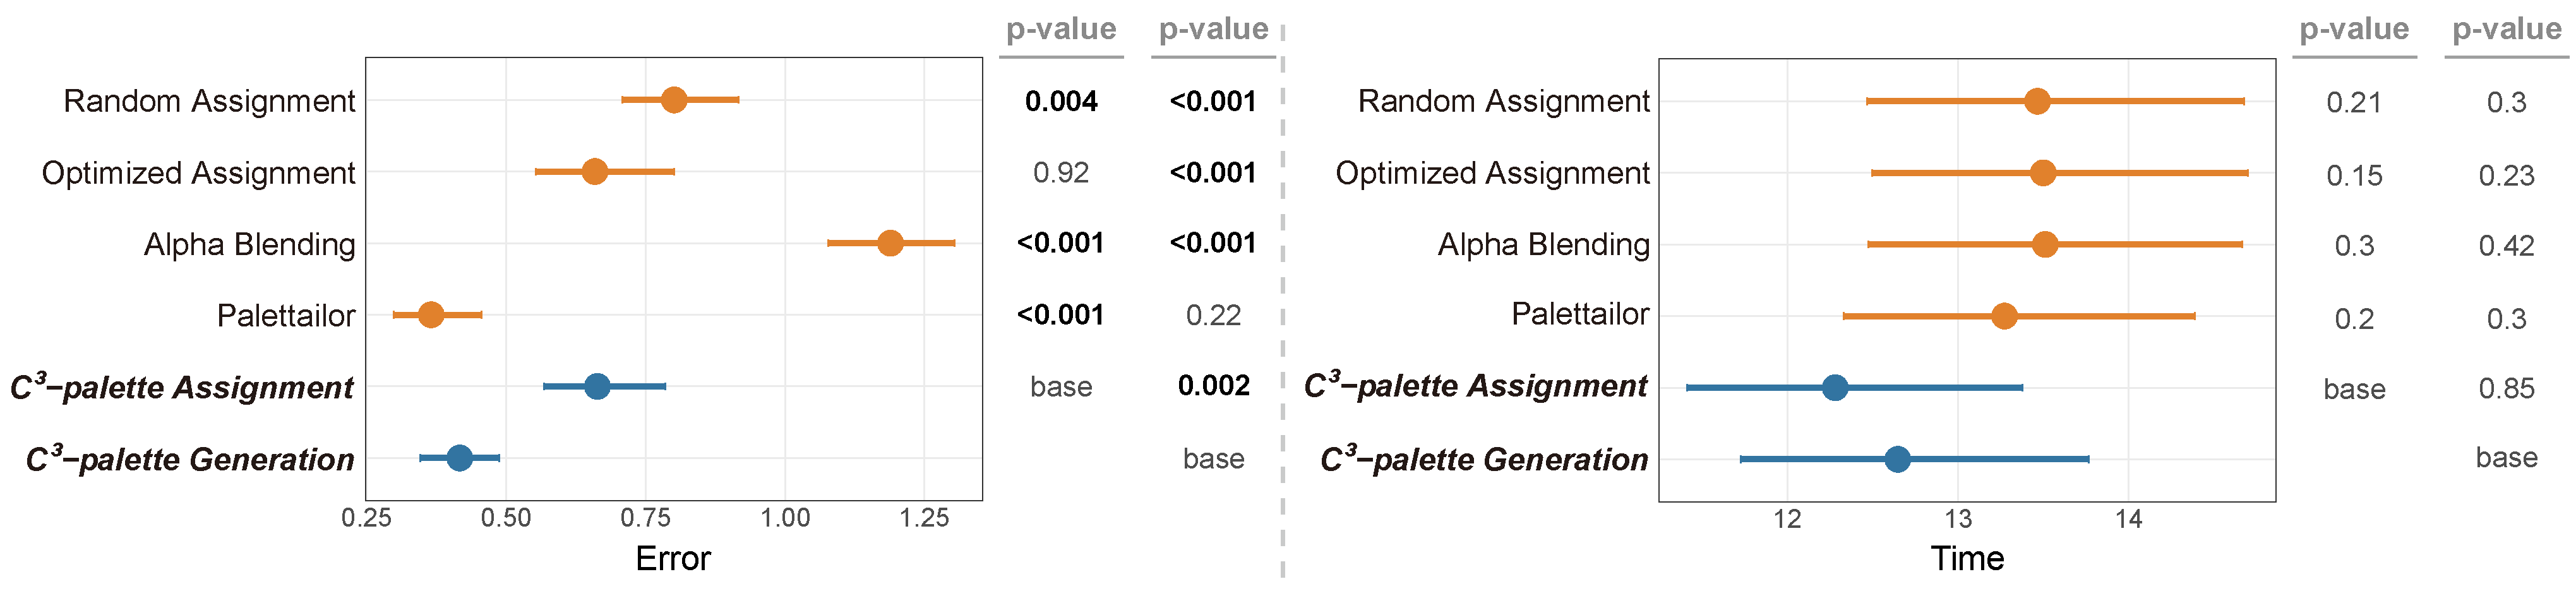
\includegraphics[width=1\linewidth]{figures/counting-results.pdf}
\caption{Confidence intervals and p-values from the Mann-Whitney test for the \emph{counting class task} of the scatterplot experiment. Error bars represent $95\%$ confidence intervals. Each p-value shows the statistical test result of one base with the other conditions. Smaller value means a better performance.}
\vspace*{-3mm}
\label{fig:counting-results}
\end{figure*}

\subsection{Discussion}
\label{subsec:discussionEval}
In summary, we evaluated the effectiveness of our approach against the benchmark conditions through three online studies, including one bar chart experiment and two scatterplot experiments.
We found that first, our method \emph{$C^3$-palette Generation} outperforms the benchmark methods on juxtaposed comparison tasks across two visualizations: bar chart and scatterplot, and specifically for the scatterplot visualization, the effects of our methods are not necessarily influenced by the change magnitude of the two scatterplots.
In addition, we observed that our \emph{$C^3$-palette Assignment} method, when coupled with a palette containing colors with a wide range of brightness and saturation, outperforms the benchmark methods. This indicates that our assignment method could perform well if given an ideal palette.
%The performance of \emph{Optimized Assignment} is comparable to \emph{Random Assignment}, this is reasonable, since the \emph{Optimized Assignment} mainly cares about the visual separability of different classes, thus it might assign the less salient color to the changed class while \emph{Random Assignment} would assign salient color even though the whole separability of the scatterplot is not very good. This also provides an explanation for the bad performance of \emph{Alpha Blending} which also assigns low contrast colors to changed classes. We show some examples for \emph{Alpha Blending} in Figs.(1,2) in the supplementary material.

Second, through the scatterplot experiments, we found that our experimental methods (\emph{$C^3$-palette Generation} and \emph{$C^3$-palette Assignment}) generally support the fundamental visual separability of the classes. It is worth noting that \emph{$C^3$-palette Generation} is not worse than \emph{Palettailor}
% which is the start-of-the-art palette generation method for visual discriminability
, while the \emph{$C^3$-palette Assignment} is not worse than the \emph{Optimized Assignment}
% which is the start-of-the-art palette assignment method for visual discriminability
. This indicates that our approach maintains the class discriminability of the scatterplot while enhances the class saliency to help user observe changes between different scatterplots.

%Third, we found that \emph{change magnitude} and \emph{change type} influence the performance of the \emph{counting class number} task. The potential explanation is that large change between scatterplots will attract participants' attention, thus make it easy to distinct different classes. This is also reasonable for \emph{change type} since point position change is easier to distinguish than point number change.
Third, for both visualizations, one of the benchmark conditions \emph{Alpha Blending} yielded a better performance in the \emph{identifying delta} tasks compared with the other benchmark methods (yet still worse than our methods), which indicates that manipulating the opacity may help people identify changes to some extent. However, when it came to the separability task, \emph{Alpha Blending} led to the worst performance of all the conditions, which indicates a tradeoff of class discriminability.
%It is obvious that the \emph{Alpha Blending} has a much higher error rate than other methods for the discrimination task. As one of the participants said, ``The ones that were harder were ones that had colors that when they overlapped would change color. It made it hard to tell if it was the same color or if it was a new color. When the colors were uniform and all the same opacity, it was much easier.'' The \emph{Alpha Blending} condition changes the opacity of unchanged classes to make them less attractive, but this will generate new color from color blending, so as to make it hard to distinct them.


There are some \textbf{limitations} within our evaluation.
%First, our experiment mainly focuses on error rate and time consumption, while other measurements were not explored, such as click order of the changed classes and time consumption for each click while \emph{cluster type} might influence the user's perception.
First, we tested the assignment of our approach using a carefully-designed and diverse palette as input (i.e., the \emph{$C^3$-palette Assignment} condition used Tableau-20), while it remains to be unclear whether other palettes (e.g., Tableau-10 or ColorBrewer) would lead to similar or different results.
Second, our experiment focused on identifying the differences between two visualizations, which is a simplified situation, since in real-world cases often more than two visualizations are compared.
Third, our evaluation focused on two visualization types: bar chart and scatterplot, while the effectiveness of our method on the juxtaposed comparison tasks of other visualizations (e.g., line chart, node-link tree) remains to be explored.
Finally, we cannot further analyze the effect of the \emph{change type}, given the current study design, though we did observe that our methods are more effective for certain types of change.
That brings us to a series of more fundamental questions: how can we properly define the types of changes? What is the just noticeable change magnitude for each change type?
Further research is needed to answer these questions so that our approach can be thoroughly evaluated.
